\documentclass[a4paper, fleqn]{article}
\usepackage{enumitem}
\usepackage{amsmath, amssymb}
\usepackage{xstring}
\usepackage{graphicx} % For including figures
\graphicspath{{./figs/}} % Path to figures
\usepackage[labelformat=empty]{caption} % To remove figure labels
% Set engineering notation
\providecommand{\sci}[1]{\protect\ensuremath{\times 10^{\StrSubstitute[0]{#1}{e}{}}}}
\setlength{\parindent}{0pt} % Set paragraph indentation to zero

\begin{document}

\underline{\textbf{Tutorial 7: Gears}}
\vspace{10pt}

\section*{In-class activities}

\begin{enumerate}
    \item A pair of gears consist of a 20 teeth pinion meshing with a 120 teeth gear. The module is 4 mm. Calculate the pitch circle of the pinion and gear, the center distance, and the gear ratio.
    \item Two modules of 3 mm gears are to be mounted on a center distance of 360 mm. The speed ratio is 1/3. Determine the number of teeth in each gear.
    \item Calculate the speed ratio for the compound chain shown below. If the input gear rotates clockwise, in which direction does the output rotate?
    
    \begin{table}[h]
    \centering
    \begin{tabular}{|c|c|c|c|c|c|c|}
    \hline
    Gear & A & B & C & D & E & F\\  
    No. of Teeth & 20 & 100 & 40 & 100 & 10 & 100\\
    \hline     
    \end{tabular}
    \end{table}

    \begin{figure}[h]
        \centering
        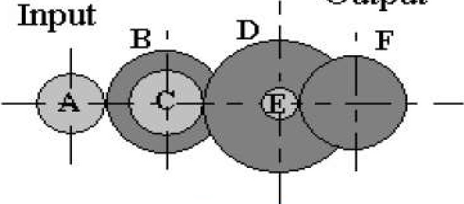
\includegraphics[width=0.5\textwidth]{t7-class1.png}
    \end{figure}
    \end{enumerate}



\section*{Theory}
\begin{enumerate}
    \item Describe the different types of gears and their applications.
    \item Discuss the importance of gear material selection and lubrication.
    \item Explain possible failure modes in gears and how to prevent them.
    \item Explain the concept of gear ratio and how it affects torque and speed.
    \item Define gear train and provide examples of its use in mechanical systems.
\end{enumerate}

\newpage
\section*{Calculations}

\vspace{10pt}
\textbf{Question 1}
\vspace{10pt}

The gears shown in Figure below have a module of 6 mm and a 20° pressure angle. Determine, and show on a free-body diagram,
\begin{enumerate}[label=(\roman*)]
    \item The tangential and radial loads on each gear.
    \item The reactions on shaft C.
\end{enumerate}
Given: Driver gear 1 transmits 80 kW at 1600 rpm through the idler to gear 3 mounted on shaft C.
\begin{figure}[h]
    \centering
    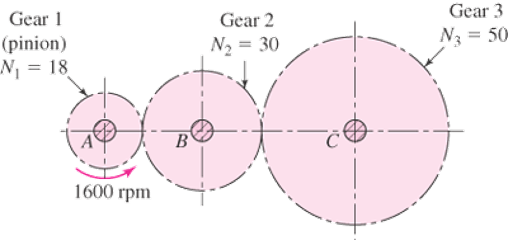
\includegraphics[width=0.5\textwidth]{t7-q1-1.png}
\end{figure}

\textbf{Solution:}\\
Given: $P=80kW$\\
$N_1=1600rpm$\\
module,$m=6mm$\\
pressure angle,$\phi=20^\circ$\\
From the figure, we have\\
$N_1=20$, $N_2=30$, $N_3=50$\\
Calculating the pitch diameter of each gear\\
$d_1=m \times N_1=108mm$\\
$d_2=m \times N_2=180mm$\\
$d_3=m \times N_3=300mm$\\

Gear 1 and 2\\
\begin{figure}[h]
    \centering
    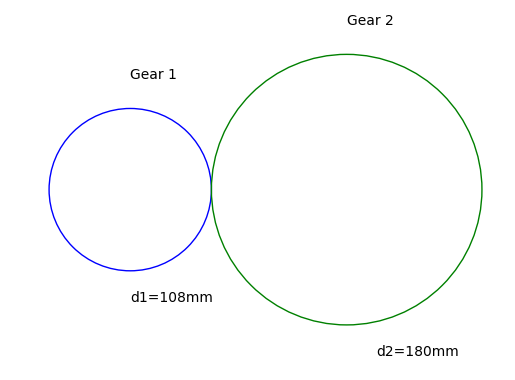
\includegraphics[width=0.5\textwidth]{t7-q1-2.png}
\end{figure}

\newpage
Draw FBD between gear 1 and gear 2\\

\begin{enumerate}
    \item Identify which one is driver and driven gear. Here, gear 1 is driver and gear 2 is driven gear.
    \item Draw rotation direction of each gear. Here, gear 1 rotates anticlockwise, therefore gear 2 rotates clockwise.
    \item Draw tangential force on \textbf{driven gear} first. Here, tangential force on gear 2 is towards up.(Follow direction of rotation)
    \item Draw radial force, Fr which is opposite to each other.
    \item Draw tangential force on \textbf{driver gear} which is opposite to driven gear. Here, tangential force on gear 1 is towards down.
\end{enumerate}

\begin{figure}[h]
    \centering
    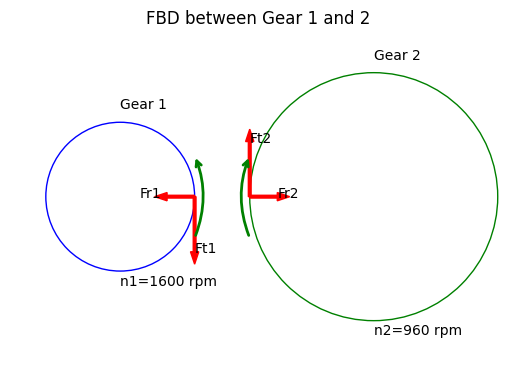
\includegraphics[width=0.75\textwidth]{t7-q1-3.png}
\end{figure}

Find torque on gear 1
\begin{equation*}
    \begin{aligned}
    P&=\dfrac{2\pi n T}{60}\\
    80000&=\dfrac{2\pi \times 1600 \times T_1}{60}\\
    T_1&=477.46 Nm
    \end{aligned}
\end{equation*}

Radius of gear 1, $r_1=\dfrac{d_1}{2}=0.054m$\\
From torque equation, we have

\begin{equation*}
    \begin{aligned}
    T_1&=F_{t1} \times r_1\\
    F_{t1}&=\dfrac{T_1}{r_1}=\dfrac{477.46}{0.054}=8841.85N
    \end{aligned}
\end{equation*}

$F_{t1}=F_{t2}=8841.85N$\\

Radial force on gear 1,

\begin{equation*}
    \begin{aligned}
    F_{r1}&=F_{t1}\tan\phi\\
    F_{r1}&=8841.85 \times \tan 20^\circ\\
    &=3218.17N
    \end{aligned}
\end{equation*}

$Fr_1=F_{r2}=3218.17N$\\

Gear 2 and 3

\begin{figure}[h]
    \centering
    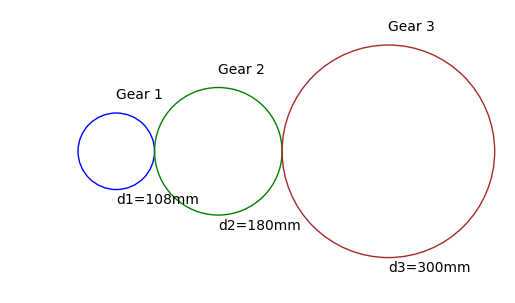
\includegraphics[width=0.75\textwidth]{t7-q1-4.png}
\end{figure}

Radius of gear 2, $r_2=\dfrac{d_2}{2}=0.09m$\\

Find speed of gear 2
\begin{equation*}
    \begin{aligned}
    \dfrac{N_1}{N_2}&=\dfrac{n_2}{n_1}\\
    \dfrac{18}{30}&=\dfrac{n_2}{1600}\\
    n_2&=960rpm
    \end{aligned}
\end{equation*}

Draw FBD between gear 2 and gear 3

\begin{figure}[h]
    \centering
    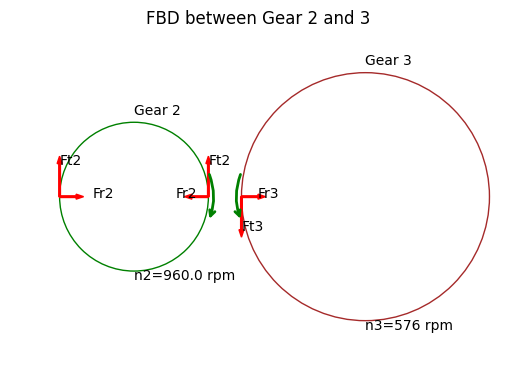
\includegraphics[width=0.75\textwidth]{t7-q1-5.png}
\end{figure}

Find torque on gear 2
\begin{equation*}
    \begin{aligned}
    P&=\dfrac{2\pi n T}{60}\\
    80000&=\dfrac{2\pi \times 960 \times T_2}{60}\\
    T_2&=795.77 Nm
    \end{aligned}
\end{equation*}

Radius of gear 2, $r_2=\dfrac{d_2}{2}=0.09m$\\

From torque equation, we have
\begin{equation*}
    \begin{aligned}
    T_2&=F_{t2} \times r_2\\
    F_{t2}&=\dfrac{T_2}{r_2}\\
    &=\dfrac{795.77}{0.09}\\
    &=8841.89N
    \end{aligned}
\end{equation*}

$F_{t2}=F_{t3}=8841.89N$\\

Radial force on gear 2,
\begin{equation*}
    \begin{aligned}
    F_{r2}&=F_{t2}\tan\phi\\
    F_{r2}&=8841.89 \times \tan 20^\circ\\
    &=3218.18N
    \end{aligned}
\end{equation*}

$Fr_2=F_{r3}=3218.18N$\\

\newpage

\textbf{Question 2}
\vspace{10pt}

In gear train shown in Figure Q2, gear 1 is the inlet of the gear train and transfers 1.8kW of power at 2400 rpm. The module of all gears in the train drive is 4 mm and the pressure angle is 20°. Diameter for gear 1, 2, 3 and 4 are 32mm, 60mm, 80mm and 100mm respectively.

\begin{enumerate}[label=(\roman*)]
    \item Determine the number of teeth for gears 1, 2, 3 and 4.
    \item Determine the tangential and radial forces between gears 1 and 2 and between
gears 3 and 4.
    \item If the diameter of gear 4 is increased to 120mm, explain how it affects the torque of gear 4
\end{enumerate}

\begin{figure}[h]
    \centering
    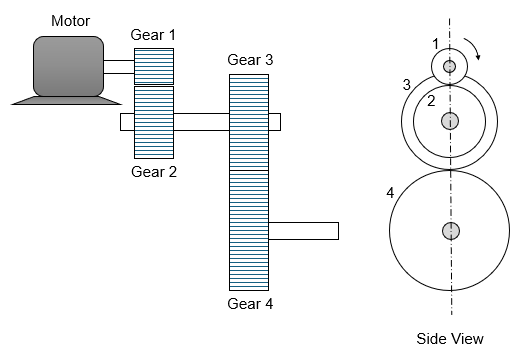
\includegraphics[width=0.5\textwidth]{t7-q2-1.png}
\end{figure}

\newpage
\textbf{Question 3}
\vspace{10pt}

The gear train in Figure Q3 is required to transmit the power of 40 kW at 1500 rpm from pinion 1. The ratio of speed between gear 1 and 2 is 5:2. Due to limited space, the ratio number of teeth on gear 3 to gear 4 is 1:3 with module of 4 mm and a pressure angle of 20. 

\begin{figure}[h]
    \centering
    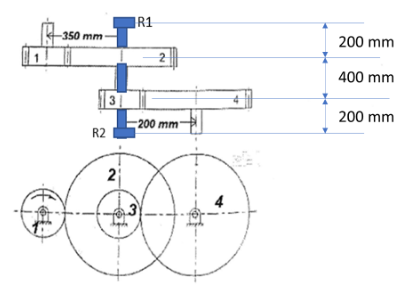
\includegraphics[width=0.75\textwidth]{t7-q3-1.png}
    \caption{Figure Q3}
\end{figure}

\begin{enumerate}[label=(\roman*)]
    \item Determine the number of teeth on gears 1,2,3 and 4
    \item Determine the radii of gears 1, 2,3 and 4
    \item Calculate the speed on gears 2, 3 and 4
    \item Determine the tangential and radial forces on each gear.
    \item Calculate the magnitude of reaction at the shaft of gear 2 and 3.
    \item Calculate the reaction at bearing R1 and R2.
\end{enumerate}

\textbf{Well-defined Questions}

\begin{enumerate}[label=(\roman*)]
    \item If the gear number 4 is reduced to 65, how does it affect gear 4 torque and speed?
    \item What happens to the gear 4 speed and torque if the teeth on gear 2 are doubled?
\end{enumerate}

\newpage

\textbf{Answer}

\textbf{Q2}

\begin{enumerate}[label=(\roman*)]
    \item $N_1=8, N_2=15, N_3=20, N_4=25$
    \item $F_{t1}=F_{t2}=447.5N, F_{r1}=F_{r2}=162.88N$\\
    $F_{t3}=F_{t4}=335.75N, F_{r3}=F_{r4}=122.2N$
    \item When the diameter of gear 4 is increased, the torque of gear 4 also increases from 16.79 Nm to 20.14 Nm.
\end{enumerate}

\textbf{Q3}

\begin{enumerate}
    \item $N_1=50, N_2=125, N_3=25, N_4=75$
    \item $r_1=100mm, r_2=250mm, r_3=50mm, r_4=150mm$
    \item $n_2=600rpm, n_3=600rpm, n_4=200rpm$
    \item $F_{t1}=F_{t2}=2546.5N, F_{r1}=F_{r2}=926.85N$\\
    $F_{t3}=F_{t4}=12732.4N, F_{r3}=F_{r4}=4634.21N$
    \item 15722.4N, $\theta=76.3^\circ$
    \item R1=5114.02N, R2=10690N
\end{enumerate}

Well-defined Questions
\begin{enumerate}[label=(\roman*)]
    \item When the number of teeth of gear 4 is reduced, the speed of gear 4 increases
from 200 rpm to 231 rpm, while the torque of gear 4 decreases from 1909.86 Nm
to 1655.21 Nm
    \item When the number of teeth on gear 2 is doubled, the speed of gear 4 decreases
from 200 rpm to 100 rpm, while the torque of gear 4 increases from 1909.86 Nm
to 3819.72 Nm.
\end{enumerate}

\end{document}